\section{Treap}

Un \textit{Treap}, también conocido como Árbol de Busqueda Binaria Aleatoreizado, es un ABB, en el que guardamos en cada nodo \(x\) una clave \(x_v\), y
un valor auxiliar llamado la \textit{prioridad} del nodo, \(x_p\). 
Estas prioridades cumplen la misma propiedad que los valores de un Heap, es decir, que la prioridad máxima de un subárbol
se encuentra en la raiz de dicho subárbol.

Si al momento de insertar un nuevo nodo, le asignamos una prioridad aleatoria,
la altura esperada del árbol resulta ser logarítmica. En particular, para toda constante \(c \in \mathbb{R}_{>0}\), la probabilidad que la altura sea mayor a \(2c \ln n\) está acotada por:

\[
\mathbb{P}[h \geq 2c \ln n] < n(n/e)^{-c \ln(c/e)}
\]

Por ejemplo, si \(n = 200000\), la probabilidad que la altura sea mayor a \(4 \ln n\) es menor que \(0.006\).

Además, si \(x\) es un nodo cualquiera, su profundidad esperada es \(\mathbb{E}[x] < 1 + 2 \ln n\). 
Por lo tanto, casi seguramente el Treap va a funcionar casi igual de rápido que otros árboles, que tienen garantías sobre la complejidad, y esto se confirma en la práctica.

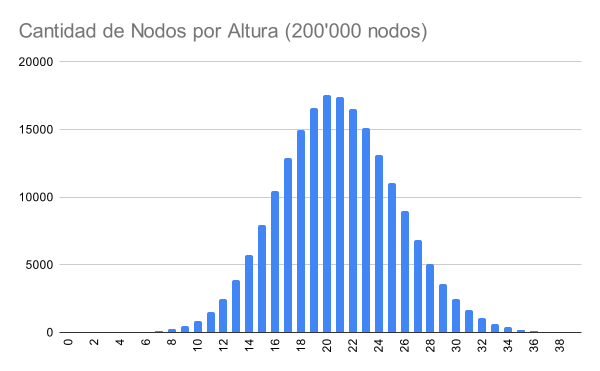
\includegraphics[width=0.8\linewidth]{Diagramas/distribucion_nodos.png}

Hay dos formas equivalentes de implementar el Treap, por eso vamos a optar por la más simple, que deriva todas las operaciones de implementar Split / Merge.

\subsection{Split}
Split(\(T, k\)) toma un Treap \(T\) y una clave \(k\), y retorna dos Treaps, \(T_\leq\) y \(T_>\), tales que:

\begin{itemize}
\item \(T_\leq \cup T_> = T\)
\item \(\forall x \in T_\leq, x_v \leq k\)
\item \(\forall x \in T_>, x_v > k\)
\end{itemize}

Es decir, particiona el Treap en dos con respecto a \(k\).
Este método va a funcionar en \(\mathcal{O}(\lg n)\) \footnote{Dado que el Treap se construye de manera aleatoria, vamos a hablar de complejidad \textit{esperada}.}, y consiste en recorrer el árbol, comparando el nodo actual con \(k\).

Si el valor en la raíz es menor o igual que \(k\), entonces la raíz y todo su subárbol izquierdo tienen que estar en \(T_\leq\), entonces partimos el subárbol derecho con respecto a \(k\), y juntamos ambas partes.
Sino, es análogo, porque la raíz y todo su subárbol derecho deben estar en \(T_>\), entonces sólo falta partir el subárbol izquierdo.

\vbox{
\begin{minted}{c++}
pair<Treap, Treap> split(Treap root, int k) {
  if (root == nullptr) return {nullptr, nullptr};
  
  if (root->key <= k) {
    auto [left, right] = split(root->right, k);
    root->right = left;
    return {root, right};
  } else {
    auto [left, right] = split(root->left, k);
    root->left = right;
    return {left, root};
  }
}
\end{minted}
}

\subsection{Merge}

De manera análoga a Split(), Merge(\(T_L, T_R\)) toma dos Treaps, el izquierdo con todos los elementos menores al derecho, y retorna un Treap con los nodos de ambos.

Tenemos que asegurar que esta operación mantenga cierto que las prioridades tienen forma de Heap.
Para esto, colocamos de raíz a la raíz del Treap con mayor prioridad.
En el caso que sea el izquierdo, hay que juntar el hijo derecho con el Treap derecho, para mantener 
el orden relativo de los nodos, para poder buscarlos a futuro.
El caso del hijo derecho es análogo, poniendo al árbol derecho de raíz, y llamando Merge() entre el árbol izquierdo, y el subárbol izquierdo del derecho.

\vbox{
\begin{minted}{c++}
Treap merge(Treap left, Treap right) {
  if (left == nullptr) return right;
  if (right == nullptr) return left;

  if (left->priority > right->priority) {
    left->right = merge(left->right, right);
    return left;
  } else {
    right->left = merge(left, right->left;
    return right;
  }
}
\end{minted}
}

Cabe destacar que, tanto Split como Merge invalidan los Treaps anteriores. 
Sin embargo, mediante \hyperref[sec:persistencia]{persistencia}, es posible mantener válidos los Treaps de input, al costo de tener que crear \(\mathcal{O}(\lg n)\) nodos adicionales.

\subsection{Insertar y Borrar}

Para insertar un nodo con valor \(x\) en el árbol, vamos a llamar a Split() dos veces,
para obtener los árboles \(T_<\), \(T_=\) y \(T_>\) (potencialmente vacíos), 
con los nodos menores, iguales o mayores que \(x\), respectivamente.

Si \(T_=\) tiene un nodo, este tiene valor igual a \(x\), y no hay que insertar nada, entonces simplemente juntamos \(T_<\) con \(T_>\).
Sino, reemplazamos \(T_=\) por un nodo nuevo con valor \(x\) (un nodo solo es a su vez un árbol),
y juntamos \(T_<\) con \(T_=\), y el resultado con \(T_>\).

Similarmente, si queremos eliminar un nodo con valor \(x\), llamamos a Split() de la misma forma,
y juntamos \(T_<\) con \(T_>\). 
Dependiendo de si el lenguaje de implementación posee un \textit{Garbage Collector} o no, puede hacer falta eliminar manualmente el nodo en \(T_=\).

\subsection[Construcción en O(n)]{Construcción en \(\mathcal{O}(n)\)}

Claramente, se puede construir un Treap en \(\mathcal{O}(n \lg n)\), 
simplemente llamando a Insert() \(n\) veces.
Sin embargo, si ya tenemos ordenados los valores iniciales a insertar, es posible reducirlo a tiempo lineal.

Primero creamos un Árbol de Búsqueda Binaria balanceado, partiendo la lista de elementos a la mitad, y llamando recursivamente. Esto es \(\mathcal{O}(n)\), ya que hacemos una cantidad constante de operaciones por nodo.

Como puede ocurrir que las propiedades no cumplan la propiedad de Heap, ahora tenemos una segunda etapa, en la que hacemos Heapify() sobre las prioridades, lo que cuesta \(\mathcal{O}(n)\), 
por ejemplo usando el algoritmo \textit{BuildHeap} de Floyd.

Nota: Incluso si los elementos no están ordenados, suele ser más rápido ordenarlos y crearlo de esta manera, porque tiene menor constante, y la altura inicial del árbol es exactamente \(\lceil \lg n \rceil\).
